\documentclass[11pt,a4paper]{article}
% RESEARCH DRAFT. Replace with the publisher's CURRENT official VJCS class
% after downloading it from World Scientific. This file compiles independently.
\usepackage[T1]{fontenc}
\usepackage[utf8]{inputenc}
\usepackage{lmodern}
\usepackage{microtype}
\usepackage[a4paper,margin=26mm]{geometry}
\usepackage{amsmath,amssymb,booktabs,tabularx,array,multirow}
\usepackage{graphicx,float,xcolor}
\usepackage{tikz}
\usetikzlibrary{positioning,arrows.meta,shapes.geometric}
\usepackage{hyperref}
\usepackage{url}
\usepackage{enumitem}
\usepackage{caption}
\usepackage{authblk}
\usepackage[numbers,sort&compress]{natbib}
\usepackage{fancyhdr}
\hypersetup{colorlinks=true,linkcolor=black,citecolor=blue!40!black,urlcolor=blue!45!black}
\setlength{\parskip}{0.35em}
\setlength{\parindent}{1.2em}
\setlength{\emergencystretch}{2em}
\setcounter{secnumdepth}{3}
\pagestyle{fancy}
\fancyhf{}
\fancyhead[L]{\small CNN--Mamba for Multi-Cancer Image Classification}
\fancyhead[R]{\small Research draft}
\fancyfoot[C]{\thepage}
\newcommand{\todo}[1]{\textcolor{red!70!black}{\textbf{[TO VERIFY: #1]}}}
\newcommand{\pending}{\textsf{PENDING}}
\newcommand{\modelname}{CNN--Mamba--CBAM--DropBlock}

\title{A Hybrid CNN--Mamba Architecture with Channel--Spatial Attention and Structured Regularization for Multi-Category Cancer Image Classification}
\author[1]{\textbf{Author Name(s) to be inserted}}
\affil[1]{Department, University/Institute, City, Country\\Corresponding author: \texttt{email@example.org}; ORCID: \texttt{to-be-provided}}
\date{Research manuscript draft --- 10 November 2026}
\begin{document}
\maketitle
\begin{abstract}
Cancer-oriented image repositories comprise heterogeneous visual categories whose reliable classification requires both local texture modeling and wider spatial-context aggregation. We describe a hybrid convolutional and selective-state-space architecture that combines four convolutional stages, channel--spatial attention, structured DropBlock regularization, and two Mamba modules. The implementation is configured for 24 image categories formed by excluding the oral-cancer subset from a public 26-category, 130,000-image compilation, yielding a nominal 120,000-image study set. Input images are resized to $224\times224$, training-only geometric augmentation is applied, and an approximately 70/20/10 image-level split is used in the supplied code. We formulate a reproducible evaluation protocol encompassing held-out classification, component ablations, calibration, and post-hoc visual attribution. \todo{Insert verified test accuracy, macro-F1, weighted one-vs-rest AUC, comparison to baselines, and a concise numerical finding after rerunning experiments.} The present draft documents the implementable method but does not claim clinical validity or unverified performance gains.
\end{abstract}
\noindent\textbf{Keywords:} Cancer image classification; CNN--Mamba; CBAM; DropBlock; Grad-CAM++; explainable AI.

\section{Introduction}\label{sec:intro}
Computational analysis of biomedical images has become a major application of computer vision. Convolutional neural networks (CNNs) are useful for learning spatially local and hierarchical visual patterns, but integrating wider contextual relationships and suppressing incidental texture cues remain important design concerns. These concerns are magnified when a benchmark pools images from different cancer-oriented collections, because source institutions, staining or acquisition protocols, backgrounds, and image modalities may vary substantially. In such settings, predictive success on a convenient random split should not automatically be interpreted as reliable disease recognition.

Recent architectures have explored complementary mechanisms for visual representation learning. Channel--spatial attention can refine convolutional feature maps \citep{woo2018cbam}, while structured regularization can inhibit dependence on small contiguous activations \citep{ghiasi2018dropblock}. Selective state-space modeling, exemplified by Mamba \citep{gu2023mamba}, provides another mechanism for propagating contextual information along a token sequence. These mechanisms motivate the architecture studied here: convolutional layers produce spatial features, two Mamba modules process the flattened spatial grids, and attention with DropBlock is inserted at intermediate feature scales.

A close example in the target journal is the breast-cancer mammography classification study by Luong \emph{et al.}, which evaluates a refined Vision Transformer against alternative CNN backbones \citep{luong2025breast}. Another relevant \emph{Vietnam Journal of Computer Science} paper by Pham \emph{et al.} constructs an integrated system for chest X-ray abnormality localization and classification and reports data preparation and comparative experiments \citep{pham2023chest}. Our application is different: it concerns a 24-way, mixed-source image categorization task rather than a single-modality mammography or thoracic-imaging task. This distinction is consequential for interpretation.

The research questions are: \textbf{RQ1}, how does the implemented CNN--Mamba hybrid perform on a properly held-out 24-category evaluation? \textbf{RQ2}, what is the individual contribution of Mamba, CBAM, and DropBlock under matched training conditions? \textbf{RQ3}, how sensitive are the results to data overlap, split construction, and input perturbations? \textbf{RQ4}, do gradient-based attribution maps provide meaningful and stable indications of decision-relevant regions?

The intended contributions are threefold. First, we specify an implementable multi-stage CNN--Mamba architecture with well-defined feature dimensions and attention/regularization placements. Second, we establish a controlled comparison and ablation plan rather than assuming that combining components guarantees improvement. Third, we define an interpretation protocol and identify limitations specific to heterogeneous, potentially duplicate-rich public image collections. \emph{Claims of statistical superiority are deferred until the proposed experiments have been executed and audited.}

\section{Related Work}\label{sec:related}
\subsection{Convolutional and transformer-based image classification}
CNNs build increasingly abstract features through convolution, nonlinear transformation, and spatial downsampling. Residual learning \citep{he2016resnet} and compound model scaling \citep{tan2019efficientnet} have provided influential baselines for modern visual classification. Vision Transformers (ViTs) instead tokenize images and apply self-attention to capture contextual interactions \citep{dosovitskiy2021vit}. In a directly relevant VJCS study, Luong \emph{et al.} report a ViT-based approach for breast-cancer X-ray image categorization and comparative evaluation against common CNN architectures \citep{luong2025breast}. These works justify benchmarking the proposed method against both a conventional CNN and at least one representative attention-based architecture, where feasible.

\subsection{Spatial attention and structured regularization}
The Convolutional Block Attention Module (CBAM) sequentially estimates channel and spatial weighting maps, reweighting a convolutional feature tensor without replacing the surrounding CNN \citep{woo2018cbam}. DropBlock removes contiguous feature regions, addressing the tendency of ordinary elementwise dropout to leave neighboring activations available as substitutes \citep{ghiasi2018dropblock}. Neither operation is novel in isolation. The empirical question is whether their placements and parameter choices benefit this data mixture when compared with parameter- and compute-aware alternatives.

\subsection{Selective state-space models for visual context}
Mamba uses input-conditioned state-space operations to process sequential representations \citep{gu2023mamba}. A two-dimensional feature map can be flattened into a sequence, processed using Mamba, and reshaped back to spatial layout. This offers a pragmatic integration strategy, although raster-scan ordering introduces spatial inductive biases and unidirectional ordering effects. The current implementation uses a single flattening order, not a multi-directional or bidirectional vision-specific Mamba design. Consequently, it should not be described as rotation-invariant or intrinsically aware of two-dimensional neighborhoods.

\subsection{Interpretability in medical-image classification}
Grad-CAM and Grad-CAM++ use class-specific gradients to visualize influential spatial features \citep{selvaraju2017gradcam,chattopadhyay2018gradcampp}. Such heatmaps are explanatory visualizations, not segmentation masks or evidence of pathologically valid localization. Without annotated regions or expert review, a heatmap's correspondence to a lesion cannot be established. Our interpretation plan therefore reports qualitative examples and recommends quantitative faithfulness or localization tests where appropriate annotations exist.

\section{Materials and Methods}\label{sec:methods}
\subsection{Dataset provenance, labels, and study population}\label{subsec:dataset}
The uploaded implementation uses \texttt{kagglehub} to retrieve the public Multi Cancer Dataset, curated by Obuli Sai Naren. The source dataset documents 130,000 images in 26 subclass folders spread over eight broad cancer-oriented collections \citep{naren2022multicancer}. Each subclass is described as containing 5,000 JPEG images. The code excludes the \texttt{oral cancer} directory, corresponding to two subclasses, and sets the output layer to 24 classes. If the downloaded dataset matches the documented version exactly, this yields 120,000 images across 24 subclasses (5,000 images each). The actual local directory traversal and per-class image counts must nevertheless be exported from a fresh dataset audit.

\begin{table}[t]
\centering\small
\caption{Expected dataset composition from the public dataset description. These are source-catalog counts, not counts demonstrated by saved notebook outputs.}
\label{tab:dataset}
\begin{tabular}{lrrl}
\toprule
Collection & Subclasses & Images & Included?\\
\midrule
Acute lymphoblastic leukemia & 4 & 20,000 & Yes\\
Brain cancer & 3 & 15,000 & Yes\\
Breast cancer & 2 & 10,000 & Yes\\
Cervical cancer & 5 & 25,000 & Yes\\
Kidney cancer & 2 & 10,000 & Yes\\
Lung and colon cancer & 5 & 25,000 & Yes\\
Lymphoma & 3 & 15,000 & Yes\\
Oral cancer & 2 & 10,000 & Excluded\\
\midrule
\textbf{Total source dataset} & \textbf{26} & \textbf{130,000} & \\
\textbf{Nominal study subset} & \textbf{24} & \textbf{120,000} & \\
\bottomrule
\end{tabular}
\end{table}

The problem is \emph{multi-category image classification}, not a single clinical cancer-detection task. Some source categories can represent normal tissue or other non-malignant findings; images also originate from different body sites or preparation methods. Consequently, predicting a dataset subclass should not be equated with establishing cancer status, subtype, prognosis, or a patient-level diagnosis. The repository's license is listed as CC BY-NC-SA 4.0; any redistribution must comply with its terms \citep{naren2022multicancer}.

\subsection{Preprocessing and data partitioning}\label{subsec:prep}
For an image $I$, the notebook constructs a $224\times224$ RGB image and applies standard tensor conversion followed by channelwise normalization using means $(0.485,0.456,0.406)$ and standard deviations $(0.229,0.224,0.225)$. The training transform adds random horizontal flipping with probability $0.5$ and random rotation within $\pm15^\circ$. Validation and test transforms contain neither random flipping nor rotation. The notebook seeds the PyTorch random splitter with 42 and uses approximately 70\% of images for training, 20\% for validation, and the remainder for testing. The \texttt{random\_split} operation rounds the first two partition sizes down; exact sample counts should be reported from the executed split.

These transformations are visible in the source code; the notebook does not preserve proof of a successful complete evaluation. Moreover, \texttt{random\_split} is not class-stratified and provides no patient-level or near-duplicate grouping. A publication-quality rerun should therefore (i) audit hashes and perceptual duplicates, (ii) group related images by patient or acquisition identity if metadata allow, (iii) stratify the final groups by class where feasible, (iv) save immutable split manifests, and (v) prevent all held-out test images from participating in architecture, hyperparameter, or checkpoint selection. If trustworthy grouping metadata are unavailable, the paper must explicitly characterize the test as \emph{image-level, source-internal} evaluation.

\subsection{Proposed CNN--Mamba architecture}\label{subsec:arch}
Let $X\in\mathbb{R}^{B\times3\times224\times224}$ be an input batch, where $B$ denotes batch size. The network consists of four convolution--batch-normalization--ReLU stages with $3\times3$ kernels, each followed by $2\times2$ max pooling. Their respective output channel counts are 32, 64, 128, and 256. CBAM and DropBlock are applied in the second and fourth stages; Mamba units operate immediately after these stages.

\begin{figure}[t]
\centering
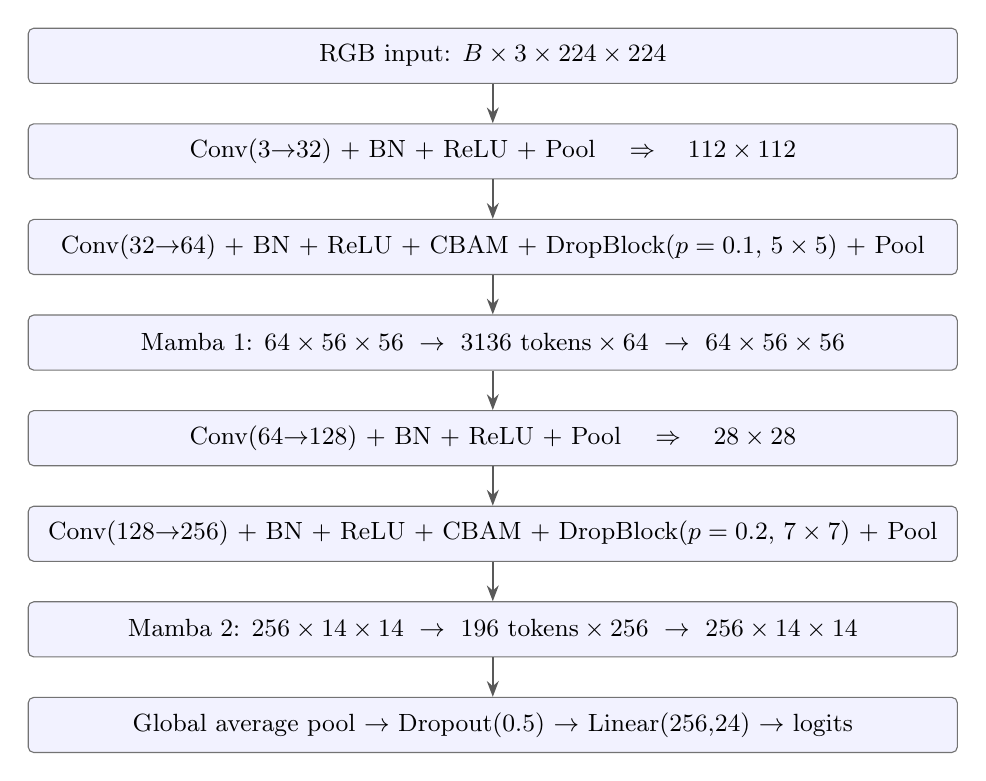
\begin{tikzpicture}[
  node distance=5mm,
  block/.style={rectangle, rounded corners=2pt,draw=black!55,fill=blue!5,minimum width=11.8cm,minimum height=0.7cm,align=center,font=\small},
  arrow/.style={-{Stealth[length=2mm]},thick,draw=black!65}]
\node[block] (in) {RGB input: $B\times3\times224\times224$};
\node[block,below=of in] (c1) {Conv(3$\to$32) + BN + ReLU + Pool $\quad\Rightarrow\quad112\times112$};
\node[block,below=of c1] (c2) {Conv(32$\to$64) + BN + ReLU + CBAM + DropBlock($p=0.1$, $5\times5$) + Pool};
\node[block,below=of c2] (m1) {Mamba 1: $64\times56\times56\ \to\ 3136\text{ tokens}\times64\ \to\ 64\times56\times56$};
\node[block,below=of m1] (c3) {Conv(64$\to$128) + BN + ReLU + Pool $\quad\Rightarrow\quad28\times28$};
\node[block,below=of c3] (c4) {Conv(128$\to$256) + BN + ReLU + CBAM + DropBlock($p=0.2$, $7\times7$) + Pool};
\node[block,below=of c4] (m2) {Mamba 2: $256\times14\times14\ \to\ 196\text{ tokens}\times256\ \to\ 256\times14\times14$};
\node[block,below=of m2] (out) {Global average pool $\to$ Dropout(0.5) $\to$ Linear(256,24) $\to$ logits};
\foreach \u/\v in {in/c1,c1/c2,c2/m1,m1/c3,c3/c4,c4/m2,m2/out}{\draw[arrow] (\u.south)--(\v.north);}
\end{tikzpicture}
\caption{Architecture reconstructed from the uploaded implementation. The feature-grid sizes assume $224\times224$ input images.}
\label{fig:architecture}
\end{figure}

\begin{table}[t]
\centering\small
\caption{Source-code architectural settings.}
\label{tab:architecture}
\begin{tabularx}{\linewidth}{lXl}
\toprule
Component & Configuration & Output spatial grid\\
\midrule
Stage 1 & Conv $3\!\to\!32$, BN, ReLU, max-pool & $112\times112$\\
Stage 2 & Conv $32\!\to\!64$, CBAM, DropBlock(0.1,5), max-pool & $56\times56$\\
Mamba 1 & $d_{\mathrm{model}}=64$, $d_{\mathrm{state}}=16$, $d_{\mathrm{conv}}=4$, expand$=2$ & $56\times56$\\
Stage 3 & Conv $64\!\to\!128$, BN, ReLU, max-pool & $28\times28$\\
Stage 4 & Conv $128\!\to\!256$, CBAM, DropBlock(0.2,7), max-pool & $14\times14$\\
Mamba 2 & $d_{\mathrm{model}}=256$, $d_{\mathrm{state}}=16$, $d_{\mathrm{conv}}=4$, expand$=2$ & $14\times14$\\
Head & Global-average pool, dropout $0.5$, 24-way linear classifier & $1\times1$\\
\bottomrule
\end{tabularx}
\end{table}

\subsection{Channel--spatial attention}\label{subsec:cbam}
For a feature tensor $F\in\mathbb{R}^{B\times C\times H\times W}$, the channel-attention branch pools over spatial coordinates using global average and maximum pooling. Both summaries are transformed by a shared two-layer $1\times1$ convolutional bottleneck with reduction ratio $r=16$. The resulting channel mask $M_c(F)$ is obtained by summation and sigmoid activation. Channel refinement and spatial refinement are then composed as
\begin{equation}\label{eq:cbam}
 F' = M_c(F)\odot F, \qquad F'' = M_s(F')\odot F',
\end{equation}
where $M_s$ concatenates channelwise average and maximum responses and applies a $7\times7$ convolution followed by sigmoid activation. This reproduces the sequential channel/spatial structure in the implementation and in CBAM \citep{woo2018cbam}.

\subsection{Spatial-sequence conversion and Mamba blocks}\label{subsec:mamba}
For $F\in\mathbb{R}^{B\times C\times H\times W}$, the feature-to-sequence operator flattens the spatial axes and transposes the result:
\begin{equation}
 T = \operatorname{Transpose}(\operatorname{Flatten}_{H,W}(F))\in\mathbb{R}^{B\times HW\times C}.
\end{equation}
Each implemented block then applies layer normalization and a Mamba operator, followed by an inverse sequence-to-image reshape:
\begin{equation}\label{eq:mamba}
 \widetilde{T}=\operatorname{Mamba}(\operatorname{LayerNorm}(T)), \qquad
 \widetilde{F}=\operatorname{Reshape}_{C,H,W}(\widetilde{T}).
\end{equation}
The notebook specifies $d_{\mathrm{state}}=16$, $d_{\mathrm{conv}}=4$, and expansion factor 2 for both units. The first unit processes 3,136 tokens with 64 channels; the second processes 196 tokens with 256 channels. The current \texttt{MambaBlock} lacks an explicit outer skip connection of the form $F+\widetilde{F}$. It therefore should not be described as a residual Mamba block without a code change.

\subsection{DropBlock and classification head}
The DropBlock layers apply structured activation suppression in training mode using $(p,b)=(0.1,5)$ and $(0.2,7)$ for stages two and four, respectively. In evaluation mode, the module follows its library-defined behavior. After the final Mamba block, global average pooling maps the $256\times14\times14$ tensor to a 256-dimensional feature vector. Dropout with probability $0.5$ precedes a learned $256\to24$ linear mapping, producing logits $z\in\mathbb{R}^{24}$. For label $y$, the training loss is multiclass cross-entropy:
\begin{equation}
 \mathcal{L}_{\mathrm{CE}} = -\frac{1}{B}\sum_{i=1}^{B}\log\frac{\exp(z_{i,y_i})}{\sum_{k=1}^{24}\exp(z_{i,k})}.
\end{equation}

\section{Experimental Design and Reproducibility}\label{sec:experiments}
\subsection{Training configuration and saved artifacts}
The uploaded notebook constructs the network in PyTorch, selects CUDA when available, configures Adam with learning rate $10^{-3}$, cross-entropy loss, and a batch size of 32. A training function supports resumable checkpoints, tracks accuracy and loss for training/validation, saves the model achieving the highest validation accuracy, and stops after three consecutive non-improving epochs by default. A notebook comment describes up to ten training epochs, but the included function invocation is commented out, and the saved notebook does not contain a completed training history. A checkpoint is loaded from a separate Kaggle model path, and a history file is read from a separate Kaggle dataset path. \todo{Provide the exact run identifier, GPU, CUDA/PyTorch/Mamba versions, epoch count, optimizer state, training duration, and checkpoint provenance.}

Reproducibility requires recording the actual image list, label mapping, hash- or group-aware split manifests, software environment, model state, optimizer state, random seeds, and training logs. Importantly, neither a fixed split seed nor an externally stored checkpoint establishes that training samples were disjoint from the current test split. The training provenance of the loaded checkpoint must be checked before making any claim about held-out evaluation.

\subsection{Baselines and controlled comparisons}
At minimum, the hybrid should be compared with: (B1) the same four-stage CNN without CBAM, DropBlock, or Mamba; (B2) the same CNN with CBAM; (B3) the same CNN with Mamba; and (B4) at least one strong external CNN baseline such as ResNet-50 or EfficientNet, trained or fine-tuned under a documented, matched protocol \citep{he2016resnet,tan2019efficientnet}. A ViT-based comparator is additionally desirable for positioning against the VJCS literature \citep{dosovitskiy2021vit,luong2025breast}. Hyperparameter tuning must use the validation set only. Report model size, inference latency, and compute budget alongside predictive metrics so differences in complexity are visible.

\subsection{Evaluation measures}\label{subsec:metrics}
Let $TP_c,FP_c,FN_c$ denote one-versus-rest confusion counts for category $c$. We calculate
\begin{align}
\mathrm{Precision}_c &= \frac{TP_c}{TP_c+FP_c}, &
\mathrm{Recall}_c &= \frac{TP_c}{TP_c+FN_c},\\
F1_c &= \frac{2\,\mathrm{Precision}_c\mathrm{Recall}_c}{\mathrm{Precision}_c+\mathrm{Recall}_c}, &
\mathrm{MacroF1} &= \frac{1}{24}\sum_{c=1}^{24}F1_c.
\end{align}
Overall accuracy is the proportion of correct predictions. Weighted-F1 averages classwise F1 using class support as the weight. One-versus-rest (OvR) area under the ROC curve (AUC) is computed for each class from its softmax probability and then aggregated with stated macro or support weights. The notebook currently prints accuracy and weighted precision, recall, and F1, and computes a weighted OvR AUC. For a balanced public compilation, macro-averaged measures and complete per-class performance are still essential. Also report 95\% bootstrap confidence intervals using an appropriate independent unit (patient or group when possible), seed-to-seed variability, and a confusion matrix with class names. Calibration and out-of-distribution evaluation are strongly recommended.

\subsection{Statistical analysis and leakage checks}
Run multiple independent training seeds on the same verified held-out split; compare paired predictions where possible rather than comparing isolated best runs. Where sample independence can be justified, paired bootstrap intervals for $\Delta$macro-F1 can quantify uncertainty. To check sensitivity to data overlap, identify exact duplicate file hashes and perceptually near-identical samples across split boundaries. Record a second, group-aware or source-aware experiment when feasible; do not silently replace an originally reported split. If patient identifiers are unavailable, state that independence from repeated patients cannot be guaranteed.

\section{Results}\label{sec:results}
\noindent\textit{Editorial status.} The notebook supplied for this manuscript does not preserve completed training curves, test predictions, test labels, computed metrics, or executed Grad-CAM++ figures. Accordingly, no accuracy or AUC value can be reported as an observed result. The tables below are structured templates to be filled only with outputs from verified experiments.

\subsection{Main held-out classification performance}
\begin{table}[h]
\centering\small
\caption{Template for held-out model comparison; values must be measured on the same test partition.}
\label{tab:main-results}
\begin{tabular}{lcccc}
\toprule
Model & Accuracy (\%) & Macro-F1 & Weighted-F1 & OvR AUC\\
\midrule
Four-stage CNN & \pending & \pending & \pending & \pending\\
ResNet-50 & \pending & \pending & \pending & \pending\\
EfficientNet baseline & \pending & \pending & \pending & \pending\\
CNN + CBAM & \pending & \pending & \pending & \pending\\
CNN + Mamba & \pending & \pending & \pending & \pending\\
\textbf{Full hybrid} & \pending & \pending & \pending & \pending\\
\bottomrule
\end{tabular}
\end{table}

\noindent\todo{Report exact held-out $N$, classification report by all 24 labels, 95\% uncertainty intervals, and the software version used to calculate metrics. Write the factual comparison only once the table is complete.}

\subsection{Learning dynamics and error profiles}
Present training and validation loss/accuracy over epochs, identifying the checkpoint-selection epoch and showing whether validation performance saturates or diverges. Provide a $24\times24$ labeled confusion matrix and distinguish cross-class mistakes within the same source collection from mistakes between visually dissimilar collections. The latter distinction is critical: classifying which source domain an image came from may be easier than recognizing pathology. \todo{Insert Figures: learning curves, full confusion matrix, clinically interpreted high-error pairs, and optional aggregate ROC curves.}

\subsection{Runtime and computational requirements}
Report GPU type, training wall-clock time, per-image inference latency at batch sizes 1 and 32, total trainable parameters, and peak GPU memory allocation. A systematic comparison is required before describing the model as lightweight, efficient, or computationally superior. \todo{Insert measured efficiency table and measurement procedure.}

\section{Ablation Study and Explainability}\label{sec:ablation}
\subsection{Component-wise ablation design}
The effects of Mamba, CBAM, and DropBlock should be tested with components removed one at a time, using the same split, train/validation protocol, and optimization budget. Where the Mamba blocks are omitted, report any change in trainable parameters and consider a capacity-matched replacement to distinguish architectural benefits from model-size effects. Changes to the CNN backbone are not necessary for a first ablation study but should be documented if introduced.

\begin{table}[h]
\centering\small
\caption{Pre-registered architectural ablation table. No experimental values are inferred.}
\label{tab:ablations}
\begin{tabular}{lccccc}
\toprule
Configuration & Mamba & CBAM & DropBlock & Macro-F1 & Params\\
\midrule
CNN only & -- & -- & -- & \pending & \pending\\
CNN + CBAM & -- & Yes & -- & \pending & \pending\\
CNN + DropBlock & -- & -- & Yes & \pending & \pending\\
CNN + Mamba & Yes & -- & -- & \pending & \pending\\
CNN + Mamba + CBAM & Yes & Yes & -- & \pending & \pending\\
Full hybrid & Yes & Yes & Yes & \pending & \pending\\
\bottomrule
\end{tabular}
\end{table}

Additional diagnostic ablations could vary Mamba placement (first block only, second block only), DropBlock probabilities and block widths, and CBAM placements. Conduct changes sequentially and report all tested settings to limit selection bias.

\subsection{Grad-CAM++-style visual attribution}
The notebook registers forward and backward hooks on the second Mamba block and computes a Grad-CAM++-style map for the predicted class. For feature activation $A^k_{ij}$ and the class-score gradient $g^k_{ij}=\partial z_c/\partial A^k_{ij}$, its implemented weighting is
\begin{align}
\alpha^k_{ij} &= \frac{(g^k_{ij})^2}{2(g^k_{ij})^2+\left(\sum_{a,b}A^k_{ab}\right)(g^k_{ij})^3+\epsilon},\\
 w_k^c &= \sum_{i,j}\alpha^k_{ij}\max(0,g^k_{ij}),\\
 L^c &= \max\left(0,\sum_k w_k^c A^k\right).
\end{align}
These equations communicate the intended weighting but are a compact approximation of the numerical implementation: the code replaces zero denominators with 1 instead of adding a literal $\epsilon$ to all denominators. This should be disclosed, and the implementation should be validated against a tested reference. It samples 20 random test images, overlays upsampled $14\times14$ maps on $224\times224$ inputs, and labels each with its true and predicted class. No attribution images are saved in the uploaded notebook. The random sample is not class-stratified and could omit important error categories.

For publication, select a predetermined stratified set of correct and incorrect predictions, include source-class context, and consider insertion/deletion or perturbation faithfulness checks. Heatmaps should not be called precise cancer-localization annotations without ground-truth lesion regions and qualified expert assessment \citep{chattopadhyay2018gradcampp}.

\section{Discussion}\label{sec:discussion}
\subsection{Interpreting any eventual performance gains}
The architecture is designed to combine local convolutional descriptors, channel--spatial weighting, structured regularization, and spatial sequence processing. The role of experiments is to determine whether these choices actually provide complementary benefits. A higher test accuracy alone would not establish the added value of Mamba unless ablations demonstrate an improvement under a comparable computational budget. Likewise, visually compelling heatmaps do not demonstrate faithful reasoning or localization of malignant tissue. Discussion of results should report both positive findings and regressions or class-specific weaknesses.

\subsection{Heterogeneous data and clinical interpretation}
Because the data are assembled from multiple anatomical domains and likely imaging conditions, a classifier may learn scanner, stain, preparation, watermark, or background characteristics that correlate with dataset source. The 24-class formulation also mixes categories that should not necessarily be considered competing diagnoses in one clinical encounter. A high source-internal score could therefore reflect dataset recognition rather than robust transfer to patient populations. External datasets, acquisition-site-held-out tests, or a narrower single-modality task would be needed to strengthen any medical relevance.

\subsection{Limitations of the current evidence}
The present notebook shows model code but not a preserved, reproducible experiment. Package-installation attempts in the saved execution trace failed for a specified PyTorch/CUDA version and for \texttt{causal-conv1d}; the subsequent Mamba import recorded an error. Later cells have no saved execution counts or outputs. This does not prove the author never trained the model elsewhere, but it prevents independent verification from this notebook alone. There is also no patient identity metadata, checkpoint provenance manifest, external test cohort, complete baseline suite, statistical confidence interval, or clinician-validated explanation study. These limitations must be addressed or explicitly reported before submission.

\section{Conclusion and Future Work}\label{sec:conclusion}
We have described a reproducible research plan for a four-stage CNN--Mamba hybrid integrating CBAM and DropBlock for 24-way categorization of images from a public multi-cancer collection. The source implementation permits precise reconstruction of feature flows, core hyperparameters, and planned evaluation steps. However, the available notebook does not establish achieved classification performance or an improvement relative to competing methods. The next stage is to audit data provenance and split independence, reproduce checkpoint-backed held-out results, run controlled ablations and external baselines, quantify uncertainty, and test attribution stability. Only after these steps can the effectiveness and potential practical relevance of the proposed combination be assessed defensibly.

\section*{Declarations}
\noindent\textbf{Data availability.} The publicly described Multi Cancer Dataset is available at \url{https://www.kaggle.com/datasets/obulisainaren/multi-cancer}, subject to its indicated license. \todo{Provide the exact version, access date, checksums, and reproducible class/split manifest.}

\noindent\textbf{Code and model availability.} \todo{Add a permanent public repository URL or explain any restrictions; include dependency lockfile, training and evaluation scripts, and validated checkpoint provenance.}

\noindent\textbf{Ethical approval and consent.} This paper describes experiments on a publicly disseminated image compilation. \todo{Confirm the original data sources, terms of reuse, de-identification, and institutional policy. Do not automatically assert IRB exemption.}

\noindent\textbf{Funding.} \todo{Insert the actual funding declaration or ``No external funding'' if true.}

\noindent\textbf{Competing interests.} \todo{Insert the authors' accurate disclosure.}

\noindent\textbf{Author contributions.} \todo{Specify each author's contributions, e.g., conceptualization, methodology, implementation, validation, writing, and supervision.}

\noindent\textbf{Acknowledgments.} \todo{Acknowledge data providers, institutional resources, and collaborators, where appropriate.}

\noindent\textbf{AI-assisted writing disclosure.} \todo{Review World Scientific's current policy and disclose any AI-assisted drafting or editing use as required; human authors are accountable for all scientific claims, citations, and analysis.}

% Self-contained bibliography for local pdfLaTeX builds without BibTeX.
% The same references are also provided in references.bib for publisher migration.
\begin{thebibliography}{11}
\bibitem{woo2018cbam} S. Woo, J. Park, J.-Y. Lee, and I. S. Kweon, ``CBAM: Convolutional Block Attention Module,'' in \emph{Proceedings of ECCV}, 2018, pp. 3--19. doi:10.1007/978-3-030-01234-2\_1.
\bibitem{ghiasi2018dropblock} G. Ghiasi, T.-Y. Lin, and Q. V. Le, ``DropBlock: A Regularization Method for Convolutional Networks,'' in \emph{Advances in Neural Information Processing Systems}, vol. 31, 2018.
\bibitem{gu2023mamba} A. Gu and T. Dao, ``Mamba: Linear-Time Sequence Modeling with Selective State Spaces,'' arXiv:2312.00752, 2023.
\bibitem{luong2025breast} H. H. Luong et al., ``An Approach for Breast Cancer X-Ray Images Classification Based on Vision Transformer,'' \emph{Vietnam Journal of Computer Science}, vol. 12, no. 3, pp. 329--347, 2025. doi:10.1142/S2196888824500210.
\bibitem{pham2023chest} V.-T.-N. Pham, Q.-C. Nguyen, and Q.-V. Nguyen, ``Chest X-Rays Abnormalities Localization and Classification Using an Ensemble Framework of Deep Convolutional Neural Networks,'' \emph{Vietnam Journal of Computer Science}, vol. 10, no. 1, pp. 55--73, 2023. doi:10.1142/S2196888822500348.
\bibitem{he2016resnet} K. He, X. Zhang, S. Ren, and J. Sun, ``Deep Residual Learning for Image Recognition,'' in \emph{Proceedings of CVPR}, 2016, pp. 770--778.
\bibitem{tan2019efficientnet} M. Tan and Q. V. Le, ``EfficientNet: Rethinking Model Scaling for Convolutional Neural Networks,'' in \emph{Proceedings of ICML}, 2019, pp. 6105--6114.
\bibitem{dosovitskiy2021vit} A. Dosovitskiy et al., ``An Image Is Worth 16x16 Words: Transformers for Image Recognition at Scale,'' in \emph{ICLR}, 2021.
\bibitem{selvaraju2017gradcam} R. R. Selvaraju et al., ``Grad-CAM: Visual Explanations from Deep Networks via Gradient-Based Localization,'' in \emph{Proceedings of ICCV}, 2017, pp. 618--626.
\bibitem{chattopadhyay2018gradcampp} A. Chattopadhyay, A. Sarkar, P. Howlader, and V. N. Balasubramanian, ``Grad-CAM++: Generalized Gradient-Based Visual Explanations for Deep Convolutional Networks,'' in \emph{WACV}, 2018, pp. 839--847.
\bibitem{naren2022multicancer} O. S. Naren, ``Multi Cancer Dataset,'' Kaggle, 2022. doi:10.34740/KAGGLE/DSV/3415848. \url{https://www.kaggle.com/datasets/obulisainaren/multi-cancer}.
\end{thebibliography}


\appendix
\section{Verification and Submission Checklist}\label{app:checklist}
The following items are not optional substitutes for evidence; they identify measurements and documentation needed to convert this honest draft into a submission candidate.
\begin{enumerate}[leftmargin=*]
 \item Export actual dataset label names, 24 class counts, sample-level hashes, and any available patient/source identifiers.
 \item Recreate train/validation/test manifests; document whether all images of an acquisition or patient stay in one partition.
 \item Verify all checkpoint weights were learned without viewing any held-out test sample, including on previous Kaggle runs.
 \item Restore runnable package versions and execute the notebook or a clean training script end-to-end; archive stdout and training history.
 \item Report actual training settings (epochs, scheduler, seeds, hardware, runtime) and per-class test predictions/probabilities.
 \item Compute accuracy, macro-/weighted F1, OvR AUC, confidence intervals, class confusion, and calibration.
 \item Train competitive baselines and component ablations with aligned training budgets and multiple seeds.
 \item Save learning curves, class-labeled confusion matrix, ROC curves, and representative correct/incorrect explanation maps.
 \item Evaluate robustness to duplicate removal and source/group-aware separation; add an external cohort if possible.
 \item Replace author/declaration placeholders; apply the current publisher LaTeX class and final journal-specific instructions.
\end{enumerate}

\end{document}
